\documentclass[12pt,a4paper]{article}
\usepackage{enumerate} %put in numbers or bullet points
\usepackage{setspace}
%\raggedright %justify the text on the left only
% NC: I removed this so you get indented paragraphs which makes it easier to read
\usepackage{graphicx} 	% For adding pictures
\usepackage{float}
\usepackage{pdflscape}	% for landscape pages
\pagenumbering{arabic}	% Page numbers
\usepackage{fancyhdr} % add headers and footers
\usepackage{hyperref} % hyper links for references

\onehalfspacing %1.5 line spacing
\usepackage[round]{natbib} % author-year citations in round brackets

%End of preamble
%--------------------------------------------------

\begin{document}

\title{Patterns of morphological evolution in tenrecs}
\author{}
\date{}
\maketitle


%Add a header 
\renewcommand{\headrulewidth}{0.0pt}
\thispagestyle{fancy}				%header on the first page only
\lhead{Sive Finlay, Progress Report}
\chead{}
\rhead{September 2014}


\section{Overview}% NC: Haven't changed much here, just corrected typos and gave some general comments. Be careful with typos. There were quite a lot and they are all highlighted by the spell check.

% NC: I wonder if this would be better framed the other way around - so start with the fact that you don't enjoy research and don't want to pursue it as a career, thus don't see any benefit to forcing yourself to complete something that would likely cause a lot of stress. Then move on to the technical difficulties? Written this way round it seems like you got overwhelmed, rather than having a better series of reasons. Also this probably doesn't need to be quite so long. You can discuss this in the meeting, and both parties are aware of your reasons. They will probably want you to re-discuss in the meeting anyway.

	My research is an investigation of evolutionary patterns in tenrecs (Afrosoricida,  Tenrecidae). The original aim of my project was to quantify both morphological and ecological diversity within tenrecs (disparity) and their similarities to other small insectivorous mammals (convergence). I have almost completed the first part of this plan; please see the paper draft `Quantifying cranial morphological disparity in tenrecs (Afrosoricida, Tenrecidae) with implications for their designation as an adaptive radiation' which accompanies this report.\\
	% NC: \\ and then a line space forces a line break between paragraphs if you think it looks neater.
	% NC: `xxx' will give you nice quotation marks
	% NC: \noindent will remove indents if you prefer
	% NC: I don't mind, I'm just showing you some stuff that you can do, it may help with the thesis

	After much careful consideration and seeking advice from many different sources, I have decided to convert my project to a research masters thesis rather than PhD. My plan is to use the attached paper as the basis for the thesis along with a complementary analysis of convergence among tenrecs and other small mammals.\\ 

	I have not made the decision to change direction lightly but I believe that it is the best option for me. If I were to continue with my project then officially I would have one year left to complete the PhD. However, realistically I know that it would take much longer. My plan was to have seven chapters: four of which would be paper driven along with introductory, data collection and conclusions chapters. The accompanying paper would be one of the four paper-driven chapters. The others would be 1) a review of methods of quantifying convergence, 2) quantifying morphological convergence among tenrecs and other small mammals using multiple methods and 3) testing whether morphological convergence is predicted by ecological similarity. In my first year report in November 2013 (see attached document) I included an outline for a further chapter based on behavioural studies of echolocatory capabilities in shrew-type (\textit{Microgale}) tenrecs. Natalie and I traveled to Madagascar in April of this year but unfortunately our experiments were unsuccessful so I was unable to collect sufficient data for this chapter.

	Completing this PhD thesis plan would be more than a simple extension of the work that I'm doing already. I would need to master different statistical techniques for quantifying convergence to a sufficient degree to be able to both use the methods for my own research and to critique them in a review. Although I'm planning to include an analysis of convergence in my masters thesis this will not be as extensive. Furthermore, to complete the PhD I would need to collect an entirely new data set of ecological variables for my species and then learn and apply different statistical methods for assessing the evidence for ecological convergences among tenrecs.

	I understand that it's common to feel overwhelmed by a PhD half way through the project. However, my decision to switch to a masters instead is not purely a matter of being overwhelmed or unwilling to approach hard work. Despite the volume of work remaining I know that I do have the ability to complete the project if necessary. However, my strengths and interests lie outside traditional research and I don't wish to continue struggling to finish a piece of work to which I'm not suited.

	I am extremely grateful to the committee for all of your help and guidance over the past two years. I feel especially thankful and fortunate to have had such a dedicated supervisor: I am so grateful to Natalie for her constant mentoring, teaching and advice and especially for her support as I was making this recent decision.  % aww 

	I would be very grateful for advice about what's the best way to approach this transition. My current plan is to contact the IRC this month (September) to tell them that I would like to terminate my contract and that they should close my research account with college.  Then I will work on finishing my paper on tenrec disparity and complete the separate analysis of convergence among tenrecs and other small mammals. Adding an introduction and discussion should not take too much longer because I have already done the majority of the background research necessary for these sections.

	My fees are covered by my final year of `Schols' so I would like to re-register as a student for this academic year and submit before the second annual deadline set by the graduate studies office on 1st of March. However, instead of allowing the write up to drag on for the best part of a year, Natalie and I have set our own deadline of submitting the thesis before the end of January (see the GANTT chart, figure \ref*{gantt}, at the end of this report for my planned timeline for completion).
 
	In this report I outline the current progress on my paper and plans for how I will develop the work into a complete Master's thesis. I have also attached a draft copy of the early stages of my thesis to demonstrate my planned structure.   


%---------------------------------------------------------------
\section{Progress on the accompanying paper}

	\textit{Journal targets: Journal of Evolutionary Biology, PLoS ONE, Journal of Mammalian Evolution?} 
\bigskip

	I have completed the majority of the work for this paper, all that remains is to develop the introduction and discussion and add a short sensitivity analysis for morphometric error checking. I plan to submit the paper by November (figure \ref{gantt}). \\
	Given that tenrecs are often cited as an example of a phenotypically diverse group \citep[e.g.][]{Olson2013}, my finding that they are not significantly more diverse than their closest relatives was unexpected and therefore should make an interesting paper.

	I would very much welcome any comments on the draft paper, particularly if you have suggestions for how I could make the overall story clearer and more interesting to a wide audience. My aim for the paper is that it is a test of a broad principle; the importance of testing our assumptions about phenotypic variation in groups that are considered to be exceptionally diverse, rather than a more limited study of shape variation in one group of mammals. I tried to put an adaptive radiation slant on my findings about tenrec morphological diversity. However, I don't have any explicit measure of the `adaptiveness' of cranial shape so I have also tried to be careful not to suggest that my analyses should be treated as a test of whether tenrecs are an adaptive radiation or not.
% NC: apostrophes get clumsy in these cases so I'd go with tenrec morphological convergence (rather than tenrecs' for simplicity of reading)

%------------------------------------------------------------------



\section{Completing the rest of the thesis} % NC: Let's give them the ToC as I suggested in my email. Also see my notes on how to separate out the sections.

	I have attached a draft copy of the early stages of my thesis to this report. I'm not asking the committee to read through the whole document but rather to refer to the table of contents to see the outline and structure of the thesis. I have already completed some of the sections and here I will outline my plans for finishing the rest of the thesis.

\subsection{Introduction}

	I will present the thesis as a general study of patterns of phenotypic diversity using tenrecs as an example.
	I will discuss disparity within the framework of how it relates to the study of adaptive radiations \citep{Losos2010a} and convergence within the context of what it tells us about the repeatability of evolution \citep[e.g][]{Blount2008}. In particular, I will stress the importance of taking quantitative approaches to studying each of these patterns rather than relying on subjective estimates. I will follow these discussions with a brief introduction of tenrecs and the long-standing interests in apparently high levels of morphological and ecological diversity within the family as well as the similarities among tenrecs and other distantly related mammal species \citep[e.g.][]{Eisenberg1969, Soarimalala2011, Olson2013}. 

	I have already completed most of the background research for this section so it will not take long to put the information together. Part of it will also be an expansion of the introduction that I have written for my disparity paper. I will add the sections on convergence and more general discussions of phenotypic diversity in October and the introduction will be completed by the end of November (figure \ref*{gantt}).

\subsection{Methods}

	This is a large section but I have completed both the work and writing for most of it already.
	I have divided the methods up into four parts: 1) museum data collection, 2) geometric morphometric analyses, 3) error checking and 4) data analysis for disparity and convergence studies (see the table of contents in the accompanying thesis draft).
%NC: again see my email comments on splitting this up
	I have finished all of sections 1 and 2 with the exception of creating diagrams to demonstrate the linear measurements which I took for skulls and limbs. For the error checking part I still need to run sensitivity analyses to test the accuracy of landmark placement on my pictures. I have all the data prepared for these analyses so they will not take long to complete. I will finish the error checking and add the results to the supplementary section of my disparity paper by the end of this month (figure \ref{gantt}).
	
	I have completed the analysis and write up for measuring morphological disparity in tenrecs (see accompanying paper).
	
	I still need to quantify convergence among tenrecs and other small mammals. I will take two approaches: estimating the amount of convergence in the tenrec phylogeny as a whole \citep{Stayton2008} and measuring the strength of convergence among specific groups of species \citep{Arbuckle2014}. These methods should be straightforward to implement because I have both the phylogenetic and morphological data prepared. 
	
	The Wheatsheaf index \citep{Arbuckle2014} measures the strength of convergence in groups which are \textit{a priori} identified to be similar. Therefore I will divide tenrecs into four separate groups and measure their morphological convergence with other small mammals. These divisions are based on the phenotypic and ecological similarities among the species and the common assumptions that tenrecs are convergent with these other groups \citep[e.g.][]{Soarimalala2011, Olson2013}. 
	
	I will compare spiny tenrecs (\textit{Echinops, Setifer, Tenrec} and \textit{Hemicentetes}) to hedgehogs, gymnures and solenodons while mole-like tenrecs (\textit{Oryzorictes}) will be compared to moles and golden moles. Most tenrecs (\textit{Microgale} genus and \textit{Geogale aurita}) are shrew-like so I will compare these species to my morphological measurements of shrews. I will also try to compare convergence within a semi-aquatic grouping of \textit{Limnogale} and \textit{Potamogale} tenrecs along with gymnures and water shrews although I may not have a sufficient sample size for this analysis. 
		
	I will complete these analyses of convergence in September and October and finish writing up the methods and results by the end of November (figure \ref{gantt}).

 
\subsection{Results}
	
	I will divide the results into two sections: disparity (results section from my paper) and convergence. I have already added my disparity results to the thesis draft.
	
	The initial output of my convergence analyses will be principal component plots showing the morphospace occupied by each of the families; tenrecs, golden moles, hedgehogs, shrews, watershrews, solenodons and moles. Figure \ref{fig:skdors_pca} is an example PCA plot for the analysis of skulls in dorsal view. These plots give a visual representation of the phenotypic similarities among my species. Each point represents the average skull shape of an individual species and distances between points indicate the morphological (dis)similarities among species.
	
	I can use these plots to calculate morphological distance matrices among species pairs. I will combine these morphological differences with phylogenetic distance matrices to generate an overall measure of the amount of convergence within the tenrec family \citep{Stayton2008} and the strength of convergence between sub-groups of tenrecs and other small mammal species \citep{Arbuckle2014}.

	I will finish writing up the results of my convergence analyses by the end of November (figure \ref{gantt}).

	%And maybe a morphological vs. phylogenetic distances plot as well?
	

  \begin{figure}[!htb]
	\centering
	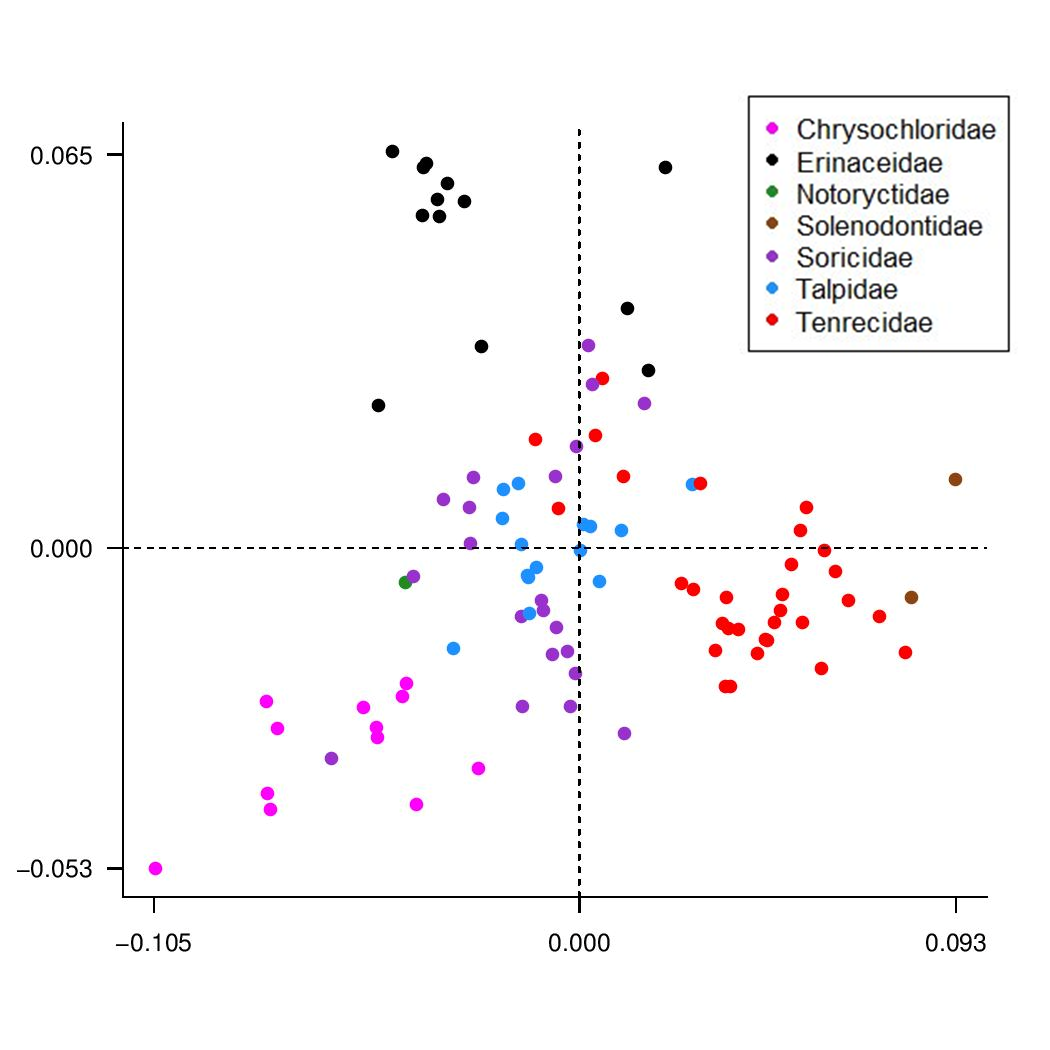
\includegraphics[width=\textwidth, height=\textheight, keepaspectratio=true]{skdors_allfam_PCA_legend.png}
		\caption{Morphospace (principal components plot) of the 		Procrustes-superimposed shape coordinates for skulls in dorsal view. Points are coloured by Family.}
	\label{fig:skdors_pca}
  \end{figure}

	

\subsection{Discussion}

	Here I will summarise my findings and interpret the results within the context of what they tell us about morphological diversity within tenrecs and the similarities among tenrecs and other small mammal species. I will also highlight the importance of taking a quantitative approach to studies of evolutionary diversity among species groups. In particular I will stress the need to apply existing methods to new groups of species which are usually not as well studied as the groups that are used to develop such metrics. %Add justification refs? 
	% NC: Think it's fine as is

	My suggestions for future directions will be based on the plans that I had made for continuing with the PhD. These will include the possibility of applying multiple metrics for measuring convergence \citep[e.g.][]{Ingram2013, Segar2013, Harmon2005}, analyses of ecological similarities to test whether there are correlations between ecological and phenotypic convergence \citep[e.g.][]{Moen2013} and the need to measure the functional importance and "adaptiveness" of convergent traits \citep{Losos2010}. I will also include a brief mention of my unsuccessful fieldwork experiments for testing echolocatory capabilities in \textit{Microgale} tenrecs and the potential for future studies of behavioural convergences among tenrecs and other small mammals.


	I will complete this section in November/December so that I will have a full thesis draft by the end of December which will leave me ready to submit by the end of January (figure \ref{gantt}).


%--------------------------------------------------------------- %I could put this back in but I didn't think it was relevant 
% NC: Up to you, might be nice to include :)
%\section{Other work}
	
	%\begin{enumerate}

	%\item \textbf{Publication since the November 2013 report}\\

	%\bigskip 
	
		%Healy, K., Guillerme T., \textbf{Finlay, S.,}, Kane, A., Kelly, S.B.A., McClean, D., Kelly, D.J., Donohue, I., Jackson, A.L. and \\Cooper, N., (2014).\\
		%Ecology and mode-of-life explain lifespan variation in birds and mammals. \textit{Proceedings of the Royal Society B, 281(1784)} 

	%\item \textbf{Presentations}\\
		%This summer I gave my first oral conference presentations at the Evolution conference in Raleigh, North Carolina (June) and the British Ecological Society Macroecology conference in Nottingham (July). I will also present my research at the Midland's Science Festival in November. 

	%\item \textbf{Reviewing}\\

		%So far I have reviewed a journal article (International Journal of Primatology) and a book chapter on phylogenetic comparative methods for quantifying convergence. I hope that I will get some more reviewing practice once I start publishing my own papers.

	%\end{enumerate}
%----------------------------------------------------------------

%GANNT chart
\begin{landscape}
  \begin{figure}[p]
	\centering
	\includegraphics[keepaspectratio=true]{Gannt_July.png}
	\caption{Timeline for completion and submission of my thesis. Tasks are colour coded according to the accompanying key}
	\label{gantt}
  \end{figure}
\end{landscape}
%-------------------------------------------------------


\bibliographystyle{jeb}
\bibliography{refs_thesis} 


\end{document}